\chapter{考察}

\section{ Small Cluster と L1$_2$ クラスターの相互作用}
18層と 24層の slub モデルについての計算結果を図\ref{fig4.1}に示す. 赤線は 24層の slub モデルのエネルギー, 緑線は 18層の slub モデルのエネルギーを示している. また, 左側の x 軸は 24層のエネルギー, 右側は 18層のエネルギーを表している. 18 層の計算では, 4 層の計算が収束しなかった. また, 8 層以降の値が判明していなかったために, その先のエネルギー傾向がどのようになるか検証する事ができなかった. そこで, 24層の slub モデルでの計算を行う事により, 4 層で計算の値が収束し, 最もエネルギーが安定するという結果が得られた. また, 8 層以降の層のエネルギー傾向は単調増加が止まり, 離した先にある別の L1$_2$ クラスターから影響を受けないという事が考察された.


\begin{figure}[htbp]
\begin{center}
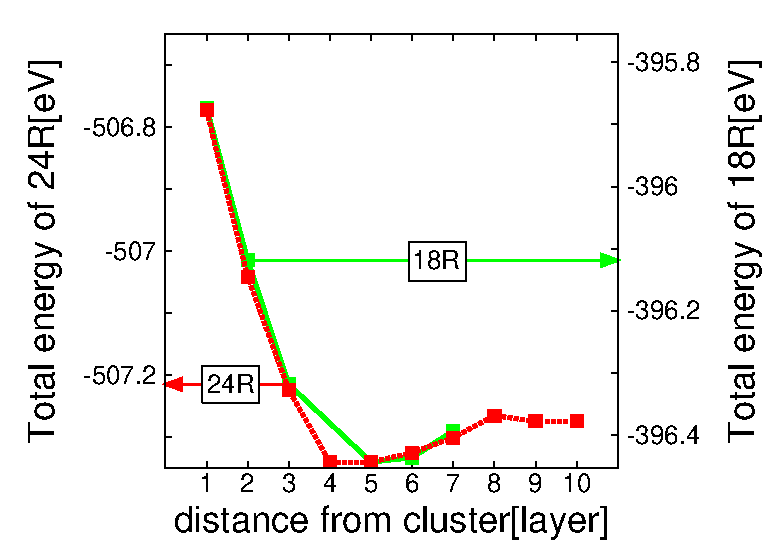
\includegraphics[width=100mm]{../consideration/smallcluster_18_24.eps}
\caption{L1$_2$ クラスターと small cluster の距離によるエネルギー変化.}
\label{fig4.1}
\end{center}
\end{figure}

\section{修正後のシナリオ}
これまでは, 溶質原子を L1$_2$ クラスターから離せば離すほどエネルギー傾向は単調減少を示し, 安定化するとされていた\cite{sakamoto}. しかし, 本研究の結果をまとめた図 3.3 のグラフは, 4 層から 5 層離れた位置でエネルギーが最安定という結果を示した. これは溶質原子が積層欠陥部から中距離離れた位置で安定化するシナリオを支持する結果となった.
この事から修正後のシナリオを以下に示す.

\begin{enumerate}
 \item Zn-Y ペアが 積層欠陥が導入されている同層に捕まる.
 \item 濃化した溶質原子が積層欠陥を誘起する.
 \item 積層欠陥が溶質原子を捕まえる.
 \item 積層欠陥ができた層でクラスターが形成される.
 \item Zn と Y の両原子が共に積層欠陥から掃き出される.
 \item 4 層程度離れた位置で溶質原子が濃化する.
 \item 2-6 の行程を繰り返す.
\end{enumerate}


\section{空孔を含んだクラスターの安定性}
今回, Small Cluster の周りで空孔が安定し, その空孔を利用したクラスター拡散が起こるのではないかという仮説のもと, 計算をおこなった. しかし, 今回の計算結果では Small Cluster から 3 層離した位置に空孔を挿入したモデルが最安定であった. これは, Small Cluster の周りに空孔が吸着し, クラスター拡散が誘発されるという仮説に反するものであった. よって, 今回の計算結果はこの仮説を支持しなかった.




